\documentclass{article}
\usepackage{graphicx}
\usepackage{subcaption}
\usepackage{multicol}
\usepackage[top=.2in, left=.2in, bottom=.2in, right=.2in]{geometry}
\begin{document}
\vspace*{\fill}
\begin{minipage}{\textwidth}
\title{Precalculus Honors Reference Sheet}
\author{Jonah Morgan}
\maketitle
\begin{multicols}{5}
\[
S_n = \frac{n}2(a_1 + a_n)
\]
\[
S_n = \frac{a_1(1 - r^n)}{1 - r}
\]
\[
S_\infty = \frac{a_1}{1 - r}
\]
\columnbreak
\[
\sum^n_{i = 1} i = \frac{n}2(1 + n)
\]
\[
\sum^n_{i = 1} i^2 = \frac{n(n + 1)(2n + 1)}6
\]
\[
\sum^n_{i = 1} i^3 = (\frac{n}2(1 + n))^2
\]
\columnbreak
\[
f'(x) = \lim_{h \to 0} \frac{f(x + h) - f(x)}h
\]
\[
\lim_{x \to 0} \frac{sin(Ax)}{Ax} = 1
\]
\[
\lim_{x \to 0} \frac{1 - cos(Ax)}{Ax} = 0
\]
\columnbreak
\[
a \cdot b = ||a|| \cdot ||b|| \cdot cos \theta
\]
\[
c^2 = a^2 + b^2 -2ab \cdot cos C
\]
\[
\frac{a}{sin A} = \frac{b}{sin B} = \frac{c}{sin C}
\]
\columnbreak
\[
r = \sqrt{x^2 + y^2}
\]
\[
x = r cos \theta
\]
\[
y = r sin \theta
\]
\end{multicols}
\end{minipage}
\begin{figure}[h]
\begin{subfigure}{.2\textwidth}
\caption{Cardioid: $1 + sin \theta$}
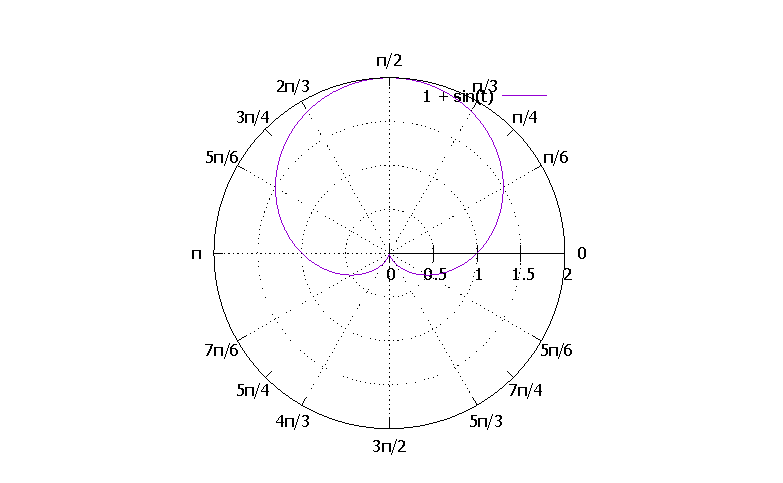
\includegraphics[scale=0.4]{cardioid.eps}
\end{subfigure}
\hfill
\begin{subfigure}{.2\textwidth}
\caption{Circle: $sin \theta$}
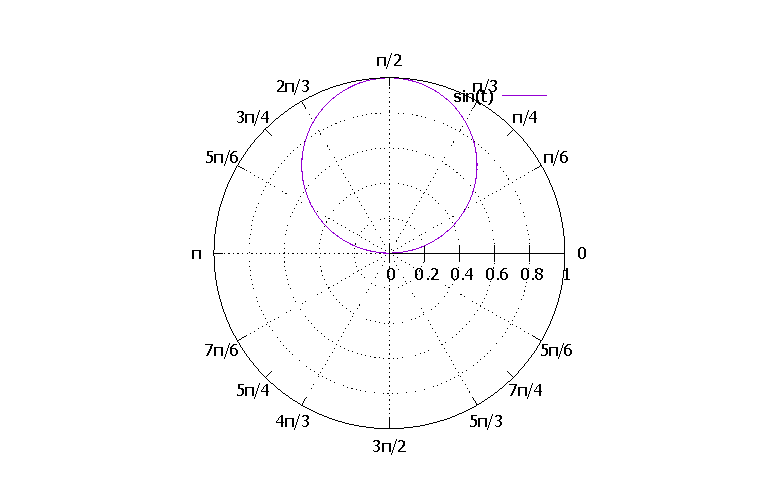
\includegraphics[scale=0.4]{circle.eps}
\end{subfigure}
\hfill
\begin{subfigure}{.2\textwidth}
\caption{Dimpled Limaçon: $2 + sin \theta$}
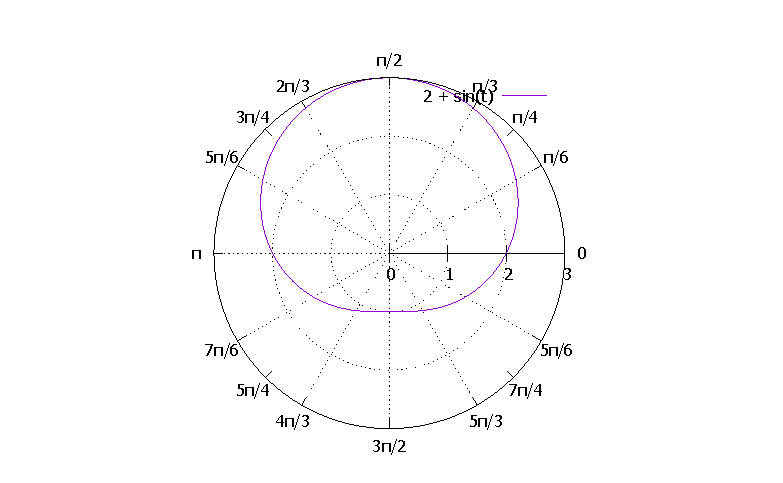
\includegraphics[scale=0.4]{dimpled-limacon.eps}
\end{subfigure}
\hfill
\begin{subfigure}{.2\textwidth}
\caption{Looped Limaçon: $1 + 2 \cdot sin \theta$}
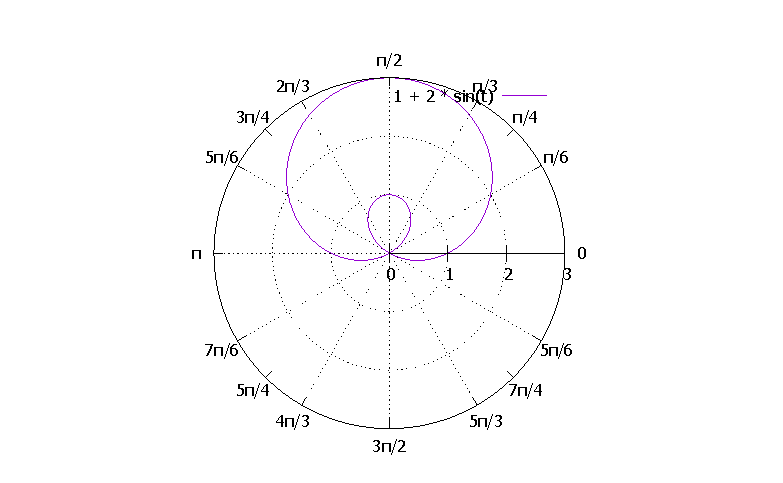
\includegraphics[scale=0.4]{looped-limacon.eps}
\end{subfigure}
\hfill
\begin{subfigure}{.2\textwidth}
\caption{Lemniscate: $\sqrt{sin 2\theta}$}
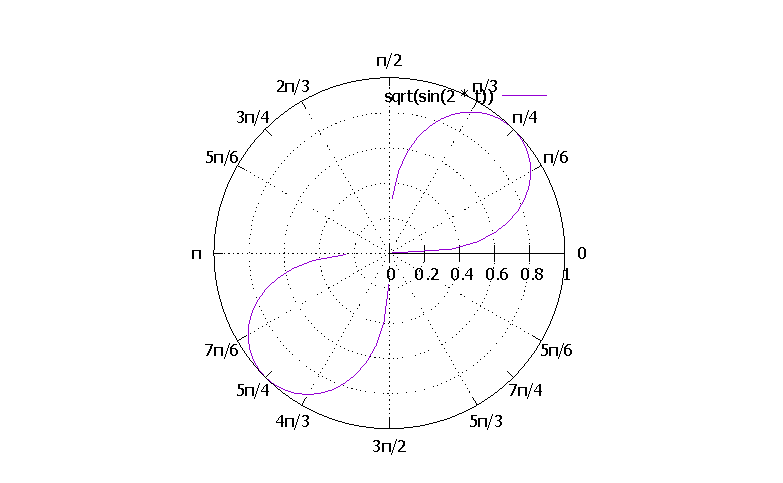
\includegraphics[scale=0.4]{lemniscate.eps}
\end{subfigure}
\hfill
\begin{subfigure}{.2\textwidth}
\caption{Rose: $sin 3\theta$}
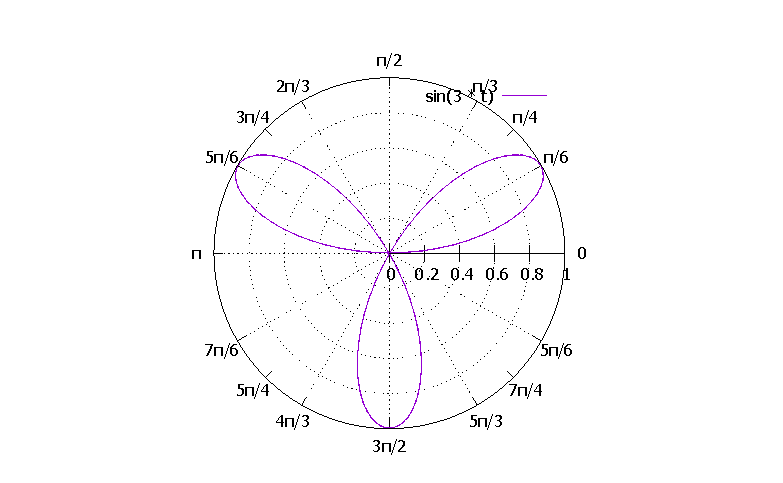
\includegraphics[scale=0.4]{rose.eps}
\end{subfigure}
\hfill
\begin{subfigure}{.2\textwidth}
\caption{Line: $\frac{1}{cos \theta + sin \theta}$}
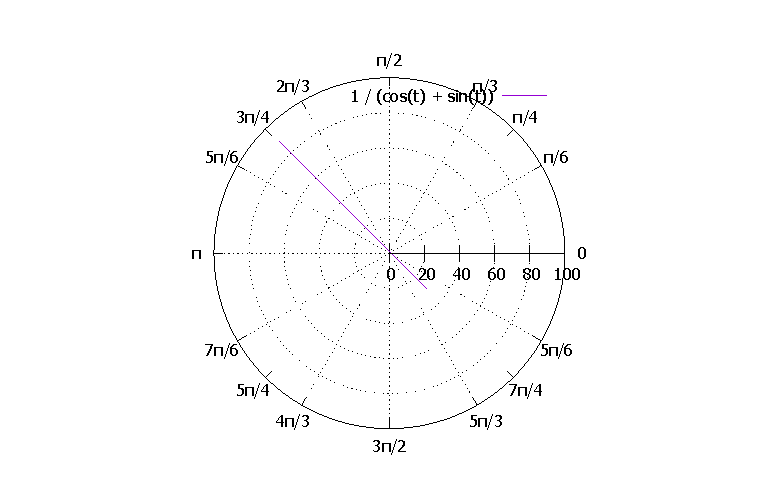
\includegraphics[scale=0.4]{line.eps}
\end{subfigure}
\hfill
\begin{subfigure}{.2\textwidth}
\caption{Parabola: $\frac{1}{1 - sin \theta}$}
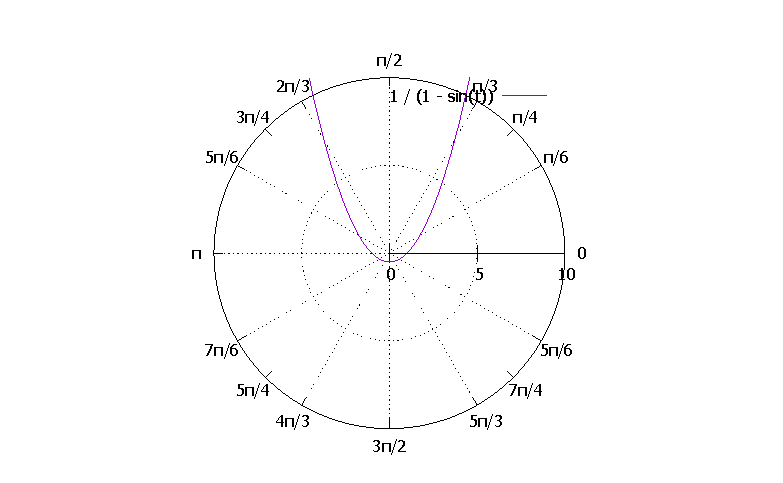
\includegraphics[scale=0.4]{parabola.eps}
\end{subfigure}
\end{figure}
\end{document}
